\documentclass[10pt,a4paper]{article}
\usepackage[utf8]{inputenc}
\usepackage[ngerman]{babel}
\usepackage[T1]{fontenc}
\usepackage{amsmath}
\usepackage{amsfonts}
\usepackage{amssymb}
\usepackage{graphicx}
\usepackage{lmodern}
\usepackage{physics}
\usepackage[left=1cm,right=1cm,top=1.5cm,bottom=1.2cm]{geometry}
\usepackage{siunitx}
\usepackage{fancyhdr}
\usepackage{enumerate}
\usepackage{mhchem}
\usepackage{mathtools}
\usepackage{graphicx}
\usepackage{float}
\usepackage[table]{xcolor}
\usepackage{mdframed}
\usepackage{csquotes}
\usepackage{trfsigns}
\usepackage{capt-of}
\usepackage{adjustbox}
\usepackage{verbatim}

\sisetup{locale=DE}
\sisetup{per-mode = symbol-or-fraction}
\sisetup{separate-uncertainty=true}
\DeclareSIUnit\year{a}
\DeclareSIUnit\clight{c}
\mdfdefinestyle{exercise}{
	backgroundcolor=black!10,roundcorner=8pt,hidealllines=true,nobreak
}

\begin{document}
\twocolumn
\pagestyle{fancy}
% \lhead{DSV Formelsammlung, Stand {\input{\string"| date + " %Y-%d-%m" \string"}}}
\lhead{Zusammenfassung System-Eigenschaften, \today}
\rhead{Sedlmeier, Toni}
\section{Elementare System-Eigenschaften}
%%%%%%%%%%%%%%%%%%%%%%%%%%%%%%%%%%%%% Elementare System-Eigenschaften %%%%%%%%%%%%%%%%%%%%%%%%%%%%%%%%%%%%%%%%%%%%
  \subsection{Statisch/Dynamisch}
  Definition \textbf{Statisches} System: (z.B ohmscher Spannungsteiler)
  \begin{mdframed}[style=exercise]
      Jedes Ausgangssignal $y(t)$ hängt zu jedem Zeitpunkt $t$ nur von den Eingangssignalen $x(t)$ zum aktuellen Zeitpunkt ab
  \end{mdframed}
  Definition \textbf{Dynamisches} System: (z.B kapazitiver Spannungsteiler)
  \begin{mdframed}[style=exercise]
      Jedes Ausgangssignal $y(t)$ hängt zu jedem Zeitpunkt $t$ von den Eingangssignalen $x(t)$ zum aktuellen und vergangenen Zeitpunkten ab
  \end{mdframed}
  %
  \subsection{Zeitkontinuierlich/Zeitdiskret}
  Definition \textbf{Zeitkontinuierliches} System:
  \begin{mdframed}[style=exercise]
    \begin{align}
      y(t)=h(t)*u(t) \ \ mit \ t \in \mathbb{R}
    \end{align}
  \end{mdframed}
  %
  Definition \textbf{Zeitdiskretes} System:
  \begin{mdframed}[style=exercise]
    \begin{align}
        y(k) &=h(k)*u(k) \\  
        k &= t\cdot T_a  \ \ k \in \mathbb{N}
    \end{align}
  \end{mdframed}


  \subsection{Linear/Nichtlinear}
  Definition \textbf{Lineares} System:
  \begin{itemize}
      \item Das Eingangssignal $u_1(t)$ verursacht das Ausgangssignal $y_1(t)$
      \item Das Eingangssignal $u_2(t)$ verursacht das Ausgangssignal $y_2(t)$
      \item Das Eingangssignal $a\cdot u_1(t) + b\cdot u_2(t)$ verursacht das Ausgangssignal $a\cdot y_1(t) + b\cdot y_2(t)$
      \item Totzeit ist \textbf{linear}
  \end{itemize}
  Bsp für \textbf{Nicht-Linearitäten:}
  \begin{itemize}
      \item $u(t)$ in Funktion $f()$ versteckt (z.b $sin, sqrt, exp$)
      \item Addition mit Konstante $k$
  \end{itemize}
  
  \begin{mdframed}[style=exercise]
    \begin{align}
        u(t)\rightarrow y(t) &= f\{u(t)\} \\
        u(t)\rightarrow y(t) &= u(t) + k
    \end{align}
  \end{mdframed}

  \subsection{Zeitvariant/Zeitinvariant}
  Definition \textbf{Zeitinvariantes} System:
  \begin{mdframed}[style=exercise]
    \begin{align}
        u(t-\tau) * h(t) = y(t-\tau)
    \end{align}
  \end{mdframed}
  Bsp für \textbf{Nicht-Zeitinvariant:}
  \begin{itemize}
    \item Multiplikation mit $f(t)$
    \item Zeitverschiebung von \textbf{nur} $u(t)$ bzw. $y(t)$
  \end{itemize}
  \begin{mdframed}[style=exercise]
    \begin{align}
        u(t) &\rightarrow y(t) = f(t)u(t)\\
        u(t) &\rightarrow y(t) = u(t-t_0)\\
        u(t) &\rightarrow y(t-t_0) = u(t)
    \end{align}
  \end{mdframed}

  \subsection{Stabil/Instabil}
  Definition \textbf{BIBO-Stabiles} System:
  \begin{mdframed}[style=exercise]
      Für ein beschränktes Eingangssignal $u(t)$ mit $\abs{u(t)} < M_1 < \infty$ 
      ist das resultierende Ausgangssignal $y(t)$ für jedes $u(t)$ ebenfalls beschränkt mit $\abs{y(t)} < M_2 < \infty$.
  \end{mdframed}
  Definition \textbf{Stabiles LTI} System:
  \begin{mdframed}[style=exercise]
      Liegen die Pole $s_\infty$ der Übertragungsfunktion $G(s)$ in der linken s-Halbebene ($Re(s_\infty) < 0$), 
      dann ist das System stabil
  \end{mdframed}

  \subsection{Kausal/Akausal}
  Definition \textbf{Kausales} System:
  \begin{mdframed}[style=exercise]
      Ein System ist kausal, wenn die Ausgangssignale $y(t)$ zu einem beliebigen Zeitpunkt $t_0$ nicht abhängen vom 
      Verlauf der Eingangssignale für $t>t_0$
  \end{mdframed}
  Die Auswirkung eines Eingangssignal kann erst nach dessen Wirkung eintreten.


\section{Darstellung von LTI-Systemen}
%%%%%%%%%%%%%%%%%%%%%%%%%%%%%%%%%%%%%  Darstellung von LTI-Systemen %%%%%%%%%%%%%%%%%%%%%%%%%%%%%%%%%%%%%%%%%%%

  \subsection{DGL im Zeitbereich}
  \begin{mdframed}[style=exercise]
    \begin{align}
        a_0y(t)+ ... + a_n \frac{d^n y(t)}{dt^n} = b_0y(t)+ ... + b_n\frac{d^n u(t)}{dt^n}
    \end{align}
  \end{mdframed}
  Bei Nichtlinearen Systemen sind $a_n$ und $b_n$ zeitabhängig $\rightarrow a_n(t) bzw. b_n(t) $


  \subsection{Zustandsraumdarstellung}
  Überführung von Eingangs-und Ausgansgrößen in Zustandsgrößen \\
\textbf{Systemgleichung:}
  \begin{mdframed}[style=exercise]
    \begin{align}
        \dot{x}(t) &= Ax(t) + bu(t)
    \end{align}
  \end{mdframed}
\textbf{Ausgangsgleichung:}
  \begin{mdframed}[style=exercise]
    \begin{align}
        y(t) &= c^T x(t) + du(t)
    \end{align}
  \end{mdframed}
  \begin{itemize}
    \item A = Systemmatrix
    \item b = Eingangsvektor
    \item c = Ausgangsvektor
    \item d = Durchgriff
  \end{itemize}
  Bei Nichtlinearen Systemen sind $A,b,c,d$ von Zustandsvariablen abhängig
  \begin{mdframed}[style=exercise]
    \begin{align}
        \dot{x}(t) &= f(x(t),u(t)) \\
        y(t) &= g(x(t),u(t))
    \end{align}
  \end{mdframed}

  \subsection{s-Übertragungsfunktion}
  \begin{mdframed}[style=exercise]
    \begin{align}
        G(s)=\frac{Y(s)}{U(s)}= \frac{b_n s^{n}+...+b_1s+b_0 } {s^{n}+...+a_1s+a_0 }
    \end{align}
  \end{mdframed}
  Laplace-Transformation ist nur für lineare, zeitinvariante Systeme definiert. (Superpositionsprinzip!)

  \subsection{G(s) Stabilität}
  Grad <= 2:
  \begin{mdframed}[style=exercise]
      Alle Koeffizienten selbes VZ $\rightarrow$ Alle NS neg. Realteil
  \end{mdframed}
  \textbf{Routh-Schema}
  \begin{mdframed}[style=exercise]
    \begin{align}
        G(s)=\textbf{1}s^5 + \textbf{8}s^4 + \textbf{28}s^3 + \textbf{58}s^2 + \textbf{67}s + \textbf{30}\\
    \end{align}
  \end{mdframed}
    \begin{center}
    \begin{tabular}{ |c|c|c|c| } 
     \hline
        $s^5$ & 1 & 28 & 67\\ 
     \hline
        $s^4$ & \textcolor{red}{8} & 58 & 30\\ 
     \hline
        $s^3$ & $-\frac{det}{\textcolor{red}{8}} \begin{pmatrix}
            1 & 28 \\
            8 & 58 
        \end{pmatrix} = 20,75$ 
        &  $-\frac{det}{\textcolor{red}{8}} \begin{pmatrix} 
            1 & 67 \\
            8 & 30 
        \end{pmatrix} = 63,25$ 
        & 0\\ 
     \hline
        $s^2$ & $-\frac{det}{20,75} \begin{pmatrix}
            8 & 58 \\
            20,75 & 63,25 
        \end{pmatrix} = 33,61$ 
        &  $-\frac{det}{20,75} \begin{pmatrix} 
            8 & 30 \\
            20,75 & 0 
        \end{pmatrix} = 30$ 
        & 0\\ 
     \hline
        s & $-\frac{det}{33,61} \begin{pmatrix}
            20,75 & 63,25 \\
            33,61 & 30
        \end{pmatrix} = 44,73$ 
         & $-\frac{det}{33,61} \begin{pmatrix}
            20,75 & 0 \\
            33,61 & 0 
        \end{pmatrix} = 0$ 
        & 0\\ 
     \hline
        s & $-\frac{det}{44,73} \begin{pmatrix}
            33,61 & 30\\
            44,73 & 0
        \end{pmatrix} = 30$ 
        & 0
        & 0\\ 
     \hline
    \end{tabular}
    \end{center}
Fertiges Schema:
\begin{center}
\begin{tabular}{ |c|c|c|c| } 
 \hline
 $s^5$ : & 1     & 28   & 67\\ 
 \hline
 $s^4$ : & 8     & 58   & 30\\ 
 \hline
 $s^3$ : & 20,75 & 63,25& 0 \\ 
 \hline
 $s^2$ : & 33,61 & 30   & 0 \\ 
 \hline
 $s^1$ : & 44,73 & 0    & 0 \\ 
 \hline
 $s^0$ : & 30    & 0    & 0 \\ 
 \hline
\end{tabular}
\end{center}
Auswertung: 
  \begin{mdframed}[style=exercise]
    \begin{center}
      VZ-Wechsel $\rightarrow$ Instabil \\
      0er-Wechsel $\rightarrow$ Nicht-BIBO-Stabil
    \end{center}
  \end{mdframed}

  \section{Nichtlineare Systeme}
  \begin{mdframed}[style=exercise]
    \begin{align}
        \dot{x}(t) = f(\ x(t), u(t)\ ) \\
        y(t) = g(\ x(t), u(t)\ ) 
    \end{align}
  \end{mdframed}
Zustandsraumdarstellung:
  \begin{mdframed}[style=exercise]
    \begin{align}
        \dot{x}(t) = A x(t)
    \end{align}
  \end{mdframed}
  \subsection{Ruhelagen und Betriebspunkte}
  Definition \textbf{Ruhelage $x_R$}:
  \begin{mdframed}[style=exercise]
    \begin{align}
        f(x_R, 0) \\ u(t) = 0
    \end{align}
  \end{mdframed}
  Definition \textbf{Betriebspunkt $x_B$}:
  \begin{mdframed}[style=exercise]
    \begin{align}
        f(x_B, u_B) \\ u(t) = u_B
    \end{align}
  \end{mdframed}
  Bestimmung Ruhelage
  \begin{enumerate}
    \item Ableitung $\dot{x}(t)$ = 0 setzen 
    \item Eingang $u(t)$ = 0 setzen 
    \item Zustand $x(t) = x_R = const.$ setzen 
  \end{enumerate}
  \begin{mdframed}[style=exercise]
    \begin{align}
        0 = A x_R 
    \end{align}
  \end{mdframed}

  \newpage
  \subsection{Stabilität nach Lyapunov}
 System in Ruhelage $x_R \rightarrow$ kleine Auslenkung $\rightarrow$ Zustand wieder in $x_R$
  \subsection{Transformation in Delta-Koordinaten}
  \begin{mdframed}[style=exercise]
    \begin{align}
        \Delta u(t) = u(t) - u_B \\
        \Delta x(t) = x(t) - x_B
    \end{align}
  \end{mdframed}
  \begin{mdframed}[style=exercise]
    \begin{align}
        \Delta \dot{x}(t) = A_B \Delta x(t) + B_B \Delta u_e(t) \\
        \Delta \dot{y}(t) = C_B \Delta x(t) + D_B \Delta u_e(t) \\
    \end{align}
  \end{mdframed}
Jacobi-Matrix $A_B$ mit $f_n$ n-te Gleichung und $x_n$ n-ter Zustand:
  \begin{mdframed}[style=exercise]
    \begin{align}
        A_B &= 
        \begin{pmatrix}
            \frac{\partial f_1}{\partial x_1} & \frac{\partial f_1}{\partial x_2} \\ \\
            \frac{\partial f_2}{\partial x_1} & \frac{\partial f_2}{\partial x_2} 
        \end{pmatrix}|_{B/RL} \\
        B_B &= 
        \begin{pmatrix}
            \frac{\partial f_1}{\partial u_e}  \\ \\
            \frac{\partial f_2}{\partial u_e}  
        \end{pmatrix}|_{B/RL} \\
        C_B &= 
        \begin{pmatrix}
            \frac{\partial g}{\partial x_1} & \frac{\partial g}{\partial x_2}  
        \end{pmatrix}|_{B/RL} \\
        D_B &= 
        \begin{pmatrix}
            \frac{\partial g}{\partial u_e}
        \end{pmatrix}|_{B/RL} 
    \end{align}
  \end{mdframed}

  \subsection{Definitheit}
  \textbf{positiv definit:}
  \begin{mdframed}[style=exercise]
    \begin{align}
        V(\Delta x)  \textcolor{red}{>} 0 \ \ \forall x \neq 0 \ \ \ und \ \ \ V(\Delta x) = 0 \ \ \forall x = 0
    \end{align}
  \end{mdframed}
  \textbf{positiv semi-definit:}
  \begin{mdframed}[style=exercise]
    \begin{align}
        V(\Delta x) \textcolor{red}{\geq} 0 \ \ \forall x \neq 0 \ \ \ und \ \ \ V(\Delta x) = 0 \ \ \forall x = 0
    \end{align}
  \end{mdframed}
  \textbf{negativ semi-definit:}
  \begin{mdframed}[style=exercise]
    \begin{align}
        V(\Delta x) \textcolor{red}{<} 0 \ \ \forall x \neq 0 \ \ \ und \ \ \ V(\Delta x) = 0 \ \ \forall x = 0 
    \end{align}
  \end{mdframed}
  \textbf{negativ semi-definit:}
  \begin{mdframed}[style=exercise]
    \begin{align}
        V(\Delta x) \textcolor{red}{\leq} 0 \ \ \forall x \neq 0 \ \ \ und \ \ \ V(\Delta x) = 0 \ \ \forall x = 0 
    \end{align}
  \end{mdframed}

  \subsection{Kettenregel}
  \begin{mdframed}[style=exercise]
    \begin{align}
        \dot{V}(\Delta x(t)) = \frac{d}{dt}V(x(t)) =\frac{\partial V}{\partial x} \cdot \frac{\partial x(t)}{\partial t}  
    \end{align}
  \end{mdframed}


  \subsection{Direkte Methode von Lyapunov}
  \begin{enumerate}
    \item Delta Transformation bestimmen
  \begin{mdframed}[style=exercise]
    \begin{align}
        \Delta \dot{x} = f (\Delta x)
    \end{align}
  \end{mdframed}
  mit Ruhelage $\Delta x = 0$
    \item Finde $V(\Delta x)$ für die gilt:
    \item $V(\Delta x)$ \textbf{positiv definit}
        \begin{itemize}
            \item $\dot{V}(\Delta x)$ nach Quadraten sortieren und schauen
            \item $\dot{V}(\Delta x)$ \textbf{negativ semi-definit} $\rightarrow$ global stabil 
            \item $\dot{V}(\Delta x)$ \textbf{negativ definit} $\rightarrow$ global asymp. stabil 
        \end{itemize}
  \end{enumerate}

  \newpage
  \subsection{Die Harmonische Balance}
  Was passiert wenn RL nicht stabil
  \begin{itemize}
    \item Zustand strebt $\rightarrow$ andere RL
    \item Zustand strebt $\rightarrow \infty$
    \item Zustand strebt $\rightarrow$ Grenzzyklus (nichtlin. Dauerschw.)
    \item Chaotisches Systemverhalten
  \end{itemize}
  Grenzzyklus = Dauerschwingung:

  \subsubsection{Grundschwingungsnäherung}

  \begin{center}
      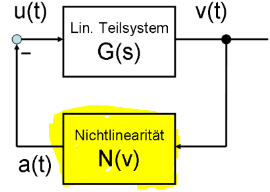
\includegraphics[width=.22\textwidth]{./img/harm1.png}
      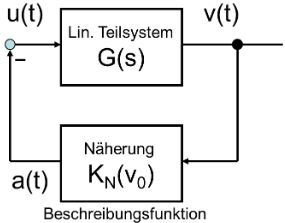
\includegraphics[width=.2\textwidth]{./img/harm2.png}
  \end{center}
  \begin{itemize}
      \item a(t) und v(t) sind cos()-Signale
      \item Ersetze N(v) durch lin. Grundschwingungsnäh. mit Verstärkung $K_N(v_0)$
      \item Wir suchen $v_0$ und $T_0$
  \end{itemize}
  $K_N(v_0)$ bewirkt Verstärkung und Phasendrehung 
  \begin{mdframed}[style=exercise]
    \begin{align}
        u(t) &= u_0 cos (w_0 t) \\
        v(t) &= v_0 cos (w_0 t + \phi_v)
    \end{align}
  \end{mdframed}

  \subsubsection{Zwei Ortkurven-Methode}
  Schnittpunkt von Lineares Teilsystem $G(j\omega_0)$ und Beschreibungsfunktion $K_N(v_0)$
  \begin{mdframed}[style=exercise]
    \begin{align}
        G(j\omega_0) = -\frac{1}{K_N(v_0)}
    \end{align}
  \end{mdframed}

  \begin{mdframed}[style=exercise]
    \begin{align}
        K_N(v_0) = \frac{a}{v_0}
    \end{align}
  \end{mdframed}

  \clearpage
  \begin{center}
      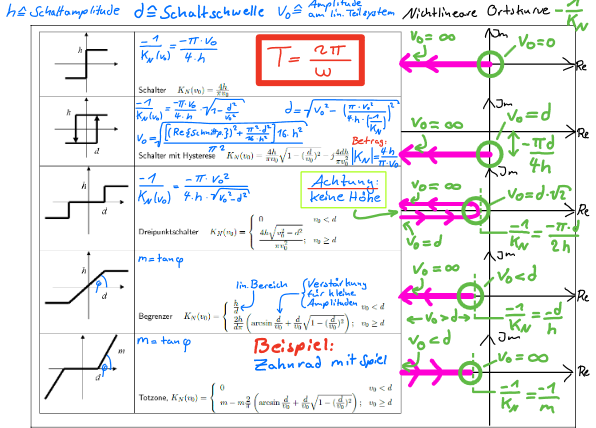
\includegraphics[width=.8\textwidth]{./img/K_N.png}
  \end{center}
\end{document}
